\paragraph{Configurable Software Systems.}
Modern software systems often need to
be customized to satisfy user requirements. Configurable software, for instance,
enables greater flexibility in supporting varying hardware platforms or tweaking
system performance. To make software systems configurable and customizable, they
exhibit a variety of \emph{configuration options}, also called
\emph{features} \citep{apel_feature-oriented_2013}.
Configuration options range from fine-grained options that tune small
functional- and non-functional properties to those that enable or disable entire
parts of the software system. The selection of configuration options can be
accommodated at different stages, either at \emph{compile-} or \emph{build-time}
when the software is built, or at \emph{load-time} before the software is
actually used.
Compile-time variability usually governs what code sections get
compiled in the program. 
Runtime-variability allows to configure the system during execution, which is
needed, for example, for context-sensitive systems. For instance, compile-time variability can be
realized by excluding code sections from compilation using preprocessor
annotations \citep{hunsen_preprocessor-based_2016} or by assembling the code
sections to compile incrementally from predefined code modules depending on the
feature selection \citep{schaefer_delta-oriented_2010}. In contrast to that,
load-time variability controls which code sections can be visited during execution. Configurations for
load-time variability can be specified using
configuration files, environment variables, or command-line arguments.
Many software systems are configurable, examples range from small open-source
command-line tools to mature ecosystems including Eclipse or even operating
systems, such as the Linux kernel with more than $11,000$ options
\citep{dietrich_robust_2012}.

Configuration options for
software systems are usually constrained (e.g., are mutually exclusive, imply
or depend on other features) to a certain extent. In the worst case though,
at which all options can be selected independently, the number of valid
configurations grows exponentially with every feature added, and exceeds
the number of atoms in the entire universe once we count $265$ independent
features. Hence, even for a small number of features, any naive approach for
assessing emergent properties of configurable software systems exhaustively for
each valid configuration is conceived infeasible. Despite this
mathematical limitation, many feasible approaches to static analysis for
configurable systems emerged. Those variability-aware approaches enable, for
instance, type checking in the presence of variability by exploiting
commonalities among different variants \citep{thum_classification_2014}.

To meet functional and non-functional requirements, users aim at finding the
optimal configuration of a configurable software system. However, this task is
non-trivial and has shown to be NP-hard \citep{white_selecting_2009}. The main
driver for the complexity are feature interactions. A \emph{feature
interaction} is an ``emergent behavior that cannot be easily deduced from the
behaviors associated with the individual features involved''
\citep{apel_feature-oriented_2013} and can make development and maintenance of
a configurable system an error-prone task.
To illustrate feature interactions, consider the following example
\citep{siegmund_performance-influence_2015}: A software system, say a file
server, is used to store files in a database and provide access upon request.
The system provides two features, encryption and compression. In
isolation, both file en- or decryption and file (de-)compression demand an
expectable fraction of memory and processor time. The performance behavior for
the software system though may vary if both features are selected. For
instance, if a file is encrypted and compressed (or vice versa), we can expect
the operation to demand less resources since an compressed file is likely to be
of smaller size than the decompressed original.
This is a positive example for a feature interaction, where the performance
behavior, although being benefiting, is unexpected.

\paragraph{Performance Behavior.}
The term ``performance'' with respect to software and software systems is not
precisely defined and differs from an end user's and developer’s perspective.
According to \cite{molyneaux_art_2014}, from a user’s perspective ``a well-performing
application is one that lets the end user carry out a given task without any
undue perceived delay or irritation''. However, to accurately assess
performance, from a practitioner’s perspective, performance is outlined by
measurements called \emph{key performance indicators} (KPIs) which relate to
non-functional requirements \citep{molyneaux_art_2014}. The set of KPIs includes
availability of a software system, its response time, throughput, and resource
utilization. Availability comprises the amount of time an application is
available to the user. Response time describes the amount of time it takes to
process a task. Throughput describes the program load or number of items passed
to a process. Resource utilization describes the used quota of resources
required for processing a task.
The performance behavior of a software system depends on the functionality
offered, the respective implementation, program load, the underlying hardware system,
environment variables, and the resulting execution. Since configuration options
control what and how functionality is executed, we concentrate here on this
source of performance. While feature interactions not necessarily cause the
software system to break severely in all cases, its overall performance can
become unfavorable for corner cases or specific configurations as the feature
selection influences the execution. 
That is, the choice of features influences the performance of a software system,
too.

\paragraph{Performance and Evolving Software.}
Actively maintained software systems evolve with every modification made, every
version released,  and patch provided. Modifications usually introduce new
functionality to the system, but functionality might as well be divided into
smaller modules to provide more fine-grained configuration options. When
features are removed from the software system, the corresponding functionality
might remain in the code base or options are merged
\citep{apel_feature-oriented_2013}.

There exists substantial work on understanding the evolution of configurable
systems, for instance, with respect to software architecture
\citep{zhang_variability_2013,passos_feature_2015} or variability
\citep{seidl_co-evolution_2012,peng_analyzing_2011,passos_towards_2012}. As
software evolves, the code base which is subject to modifications and the
overall architectural quality can degrade. Common symptoms of architectural
degradation are code tangling and scattering
\citep{zhang_variability_2013,passos_feature_2015}, which lead to less cohesive and stricter coupled code. 
The more the code base is constrained and interdependent, the more software can become ``brittle'' \citep{perry_software_1991}, less flexible, harder to adapt, and therefore harder to evolve.
Evolution of software, especially with respect to variability, is essentially
driven by and can be conceived as adapting a software system to changed
requirements and contextual changes \citep{peng_analyzing_2011}. That is,
(potential) degradation of software quality as software evolves is often a phenomenon due
to decisions trading quality assurance (QA) and maintenance tasks with meeting
requirements and schedules \citep{guo_tracking_2011}. The metaphor of
\emph{technical debt} \citep{guo_tracking_2011} which is commonly used to
describe this trade-offs and corresponding costs, outlines the risk that postponed maintenance tasks pose to
software evolution. Although every deferred maintenance or QA task may save
some cost, it also could have unveiled software defects
in the first place. Technical debt implies both interest, so to speak, the
potential damage of a defect depending on its severity, as well as the
probability of incurring interest. A defect can be severe, yet fixable with
reasonable effort and cost. However, the aforementioned symptoms of
architectural degradation and deferring maintenance render bug-fixing to become
more and more expensive.

Besides the aspects of software evolution discussed above, the evolution of
performance for software systems has gained more attention recently. In
practice though, quality assurance with respect to performance is still
conducted to an unsatisfactory extent, or accommodated too late in the
development process, according to \cite{molyneaux_art_2014}. Thus, postponed
maintenance and QA with respect to performance is likely to a driving factor for
degradation of performance quality, or simply called \emph{performance regression}.

While performance engineering has emerged as a discipline of or target
in software testing, qualitative root-cause analysis, for the most part, is
still conducted manually \citep{molyneaux_art_2014}. However, there exists work
on automated root-cause analysis for performance bugs, such as measuring the
execution time of unit tests, whereby an increased execution time indicates performance
regression, and the corresponding unit test helps isolating the root-cause
thereof \citep{heger_automated_2013,nguyen_industrial_2014}. In conclusion, we
see that, to better assure good software performance, more knowledge about performance behavior needs to be
available, ideally, earlier in the development process.

\paragraph{Performance Prediction.}
For configurable software systems, performance behavior can be more complex and
dependent on the feature selection, as we have seen with the example for
feature interactions above. Similarly, quality assurance for configurable
software systems is far from exhaustively testing all possible configurations,
but rather close to only testing a selection of configurations sampled with
respect to certain constraints. Sampling strategies might stress feature
interactions, such as pair-wise sampling \citep{siegmund_predicting_2012}.
However, all samples are selected with the intention to learn as much as
possible about the entire system from a small sample set of variants. So to
speak, a sampling strategy is ``optimal'' if for a resulting sample set, the
probability of missing an arbitrary (relevant) feature interaction, is minimal.

While performance testing is apparently useful, recently, a number of techniques
to model and predict performance behavior for arbitrary configurations have
emerged
\citep{siegmund_predicting_2012,siegmund_performance-influence_2015,guo_variability-aware_2013,sarkar_cost-efficient_2015}.
The underlying optimization problem of performance-prediction models is to find an accurate estimator $\hat{f}$ for a function $f$ describing a performance
property depending on the feature selection. Performance properties can be
estimated without performance measurements, for instance by inferring
performance properties from software models \citep{woodside_future_2007};
measurement-based approaches for configurable systems address this optimization
problem.  The proposed approaches include learning performance behavior with decision trees
\citep{guo_variability-aware_2013,sarkar_cost-efficient_2015}, learning a frequency-based representation
of the target function \citep{zhang_performance_2015}, or learning the
influence of single features and all performance-relevant feature interactions
\citep{siegmund_predicting_2012,siegmund_performance-influence_2015}. All
approaches have shown promising error rates for several real-world applications
and allow prediction of system performance for arbitrary configurations.
To create performance-prediction models, all approaches demand samples of
performance measurements for multiple configurations.

\section{Problem Statement}
The assessment of performance evolution requires a series of
performance-prediction models describing performance behavior for a series of
versions of a corresponding configurable software system. Assessing the
performance behavior for a single version of a configurable software system entails a number of
necessary and preliminary tasks. However, these tasks become even more
complicated once a series of versions needs to be assessed:
\begin{itemize}

  \item \emph{Variability Model Synthesis:} Not all configurable software
  systems do explicitly exhibit a variability model which is, however, required to derive
  all valid variants \citep{rabkin_static_2011,nadi_where_2015}.
	While substantial work exists on reverse engineering variability models from
	code
	\citep{rabkin_static_2011,she_reverse_2011,zhou_extracting_2015,nadi_where_2015}
	 or non-code artifacts
	\citep{alves_exploratory_2008,andersen_efficient_2012,bakar_feature_2015}, many
	techniques still involve manual decisions \citep{she_reverse_2011} and domain
	knowledge \citep{nadi_where_2015}.
	Moreover, variability models evolve as part of the software
	\citep{peng_analyzing_2011}, vary from version to version, and therefore,
	require repeated reverse engineering steps.
	
	%\item \emph{Configuration Translation:} The translation of a valid
	%%configuration to a configuration artifact such as a configuration file or a
	%list of command-line arguments usually differs from system to system. This
	% step may be automated, but one still needs to detect how configurations are read by the software system one wants to study.

%\item \emph{Automated Integration:} The sampe challenge applies to the
%%infrastructure when we need to compile or build a software system for a
% specific configuration since there exist many possible build tools such as makefiles.
%Again, the build process can be automated, but one needs to detect and
%specify the build mechanism used and relate it to a specific configuration.

\item \emph{Version Sampling:} To study performance evolution, we need to
specify which snapshots or versions of a software system are relevant to
describe its performance behavior over time. While detecting releases and release candidates should be straightforward, one might, for instance, be interested in the performance evolution including snapshots
between two releases, for example after bug fixes. Since it is  often the case
that not all snapshots do compile, classifying defect snapshots can still be tedious work.

\item \emph{Performance Assessment:} The accurate assessment of
performance evolution requires a suitable testing setup. The methodology required for assessing performance
among others requires the selection of suitable performance metrics and
corresponding benchmarks, means to record measurements, and repeat experiments
easily as well as proper ways to interpret and compare results.
\end{itemize}

\paragraph{Goals and Thesis Structure.}
The goal of this thesis is to provide a theoretical and practical methodology to enable
exhaustive performance measurements of configurable software systems and over
their version history. That is, we contribute a guideline of and tool support
for performance measurements of configurable and evolving software systems. Our
research objectives and desired outcomes are

\begin{itemize}
\item a literature overview regarding software evolution, feature model
synthesis, and performance assessment,
\item a methodology to assess performance evolution with respect to the
aforementioned challenges, and
\item a practical tool for performance measurement for multiple revisions of
configurable software systems.
\end{itemize}

We also propose an approach of automatically detecting promising versions of the
configurable software systems for performance measurements and evaluate whether
our assumptions hold. \\


\section{A Methodology for Assessing Performance Evolution}
The methodology described in this thesis is organized with respect to three
dimensions of configurable software systems: \emph{variability}, \emph{version
history}, and \emph{performance}. The schematic overview of the performance
evolution assessment process shown in Figure~\ref{fig:overview} outlines the major aspects of each
dimension.

\begin{figure}[h!]
	\centering
	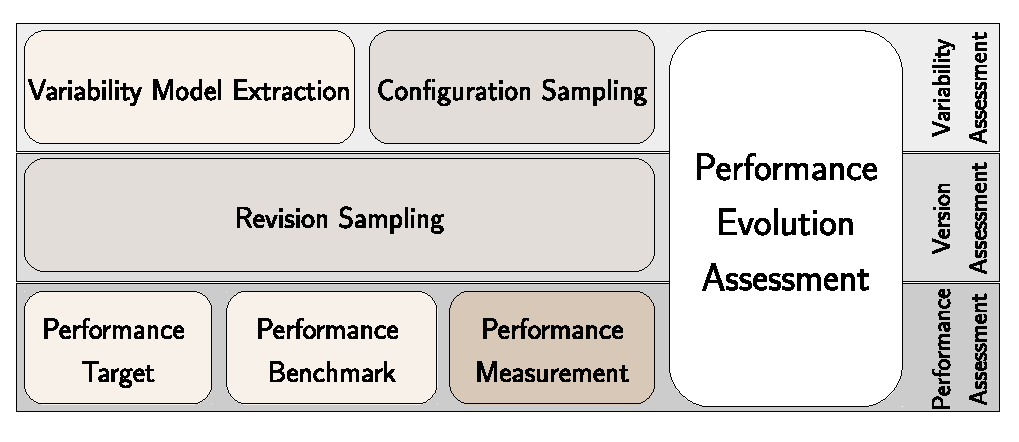
\includegraphics[width=0.99\textwidth]{images/process_overview.eps}
	\caption{Overview of the the proposed methodology including the necessary processes.}
	\label{fig:overview}
\end{figure}

First, objectives related to the variability of a configurable software system
are considered. This includes the extraction and comprehension of knowledge
about the system’s variability. Second, we address objectives which emerge with
evolving software, for instance whether a system compiles for a specific
version, or whether a version is a promising candidate for detecting
performance changes. Finally, we describe in detail the assessment of
performance which comprises the selection of suitable performance benchmarks as
well as a selection of appropriate statistical means to summarize, compare, and
evaluate performance statistics in order to derive meaningful insights.

In addition to the three aforementioned dimensions in Figure~\ref{fig:overview},
performance evolution assessment can also be conceived as consisting of three different
categories of tasks, as the different colorizations indicate. 
First, for a configurable software system, its variability needs to be
assessed in order to obtain a variability model to derive and
select configurations from.
Second, for a software system, a sample set of revisions needs to be selected.
Since covering all variants and versions is not feasible, a sampling strategy needs to be chosen
which is likely to uncover performance changes. Finally, the
performance assessment goals are specified and corresponding
measurements are conducted and evaluated as mentioned above. \\

The thesis is organized as follows. Chapter\,\ref{chapter:2} provides the
background to the relevant topics discussed in this thesis, including variability modeling,
software evolution, variability model synthesis, performance assessment,
statistical basics to summarize data records, and performance prediction
models. In addition, we review existing work related to the thesis topic.
In chapter\,\ref{sec:chapter:3}, we review existing approaches to understanding and
comprehending variability in configurable software systems. We categorize and
summarize methodological strategies to synthesize variability models and
discuss different configuration sampling strategies.
In chapter\,\ref{chapter:4}, we construct and evaluate methodological strategies to
select revisions likely to have an impact on performance from the overall
version history to sketch performance evolution efficiently.
In chapter\,\ref{chapter:5}, we propose our performance measurement methodology along
with statistical considerations regarding the summarization and presentation of
measurements results.
In Chapter\,\ref{chapter:6}, we evaluate several aspects of our tool with respect to
practicality and discuss the results thereof. 
Finally, chapter\,\ref{chapter:7} concludes the thesis and gives an outlook on
possible future work.
